\documentclass[a4paper, 12pt]{article}
\usepackage{geometry}
\geometry{a4paper,
total={170mm,257mm},left=2cm,right=2cm,
top=2cm,bottom=2cm}

\usepackage{mathtext}
\usepackage{amsmath}
\usepackage[T2A]{fontenc}
\usepackage[utf8]{inputenc}
\usepackage[english,russian]{babel}
\usepackage{graphicx, float}
\usepackage{tabularx, colortbl}
\usepackage{caption}
\captionsetup{labelsep=period}

\newcommand{\parag}[1]{\paragraph*{#1:}}
\DeclareSymbolFont{T2Aletters}{T2A}{cmr}{m}{it}
\newcounter{Points}
\setcounter{Points}{1}
\newcommand{\point}{\arabic{Points}. \addtocounter{Points}{1}}
\newcolumntype{C}{>{\centering\arraybackslash}X}

\author{Калинин Даниил, Б01-110}
\date{\today}
\title{Лабораторная работа 4.7.1. Двойное лучепреломление}

\begin{document}
\maketitle
\parindent=0cm

\parag {Цель работы}
Изучение зависимости показателя преломления необыкновенной волны от направления двоякопреломляющем кристалле; определение главных показателей преломления $n_0$ --- обыкновенной и $n_e$ --- необыкновенной волны в кристалле наблюдение эффекта полного внутреннего отражения.

\parag {В работе используются}
Гелий-неоновый лазер, вращающийся столик с неподвижным лимбом, призма из исландского шпата, поляроид.

\parag {Теоритическая справка} ~\\

При падении световой волны на границу изотропной среды в этой среде от границы распространяется одна волна. Если среда анизотропна, то в ней в общем случае возникают две волны, распространяющиеся от границы в разных направлениях и с разными скоростями. Это явление называется двойным лучепреломлением.~\\

\textbf{Двойное лучепреломление в призме исландского шпата}~\\

    \begin{figure}
        \begin{center}
        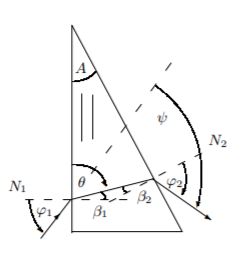
\includegraphics[width = 0.3\textwidth]{light_way.png}
        \end{center}
        \caption{Ход луча в призме}
    \end{figure}
    При таком ходе луча и расположении призмы можно посчитать показатель преломления изотропной среды по формуле

    \begin{equation*}
        n = \frac{\sin\left(\frac{\psi_m + A}{2}\right)}{\sin \left(\frac{A}{2}\right)}
    \end{equation*}
    
    Здесь $\psi_m$  --- минимальный угол, на который призма преломляет луч.
    Если призма неизотропна, то этой формулой, строго говоря, можно воспользоваться только для обыкновенной волны, которая распространяется так же, как и в изотропной среде. 
    
\parag {Экспериментальная установка}~\\

\begin{figure}[H]
    \centering
	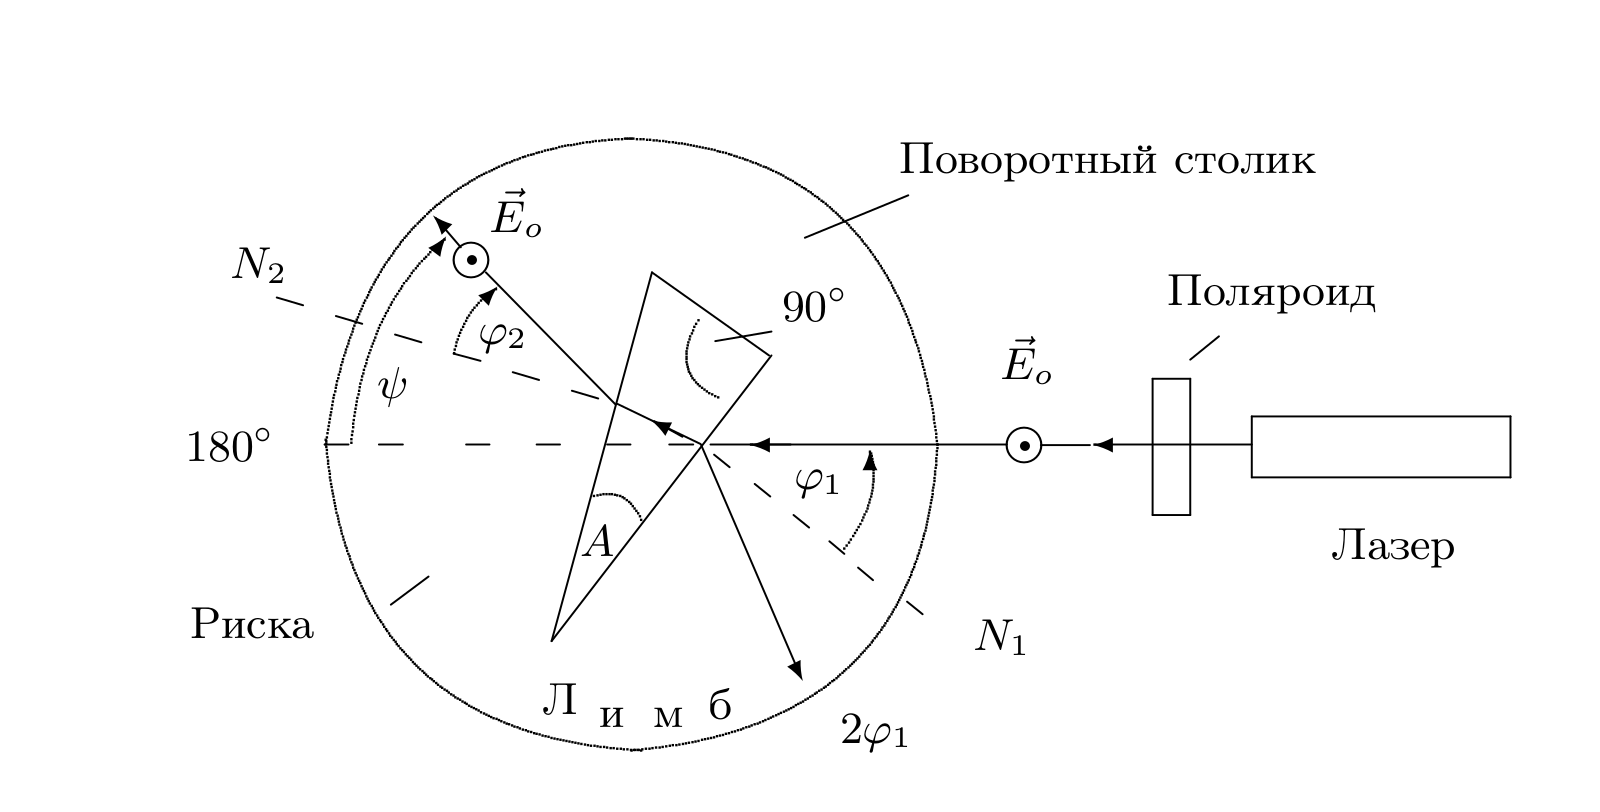
\includegraphics[width = 0.7\linewidth]{setup.png}
	\caption{Схема экспериментальной установки}
\end{figure}	


\parag {Ход работы} ~\\
    \point Отъюстируем установку. Для этого отцентруем экран по лучу лазера, то есть убедимся, что луч проходит под отметками $0$ и $180$.

    \point Установим луч, отраженный от большего катета в $10^\circ$, тогда риска указывает на $\varphi_0 = 65^\circ$.

    \point  Установим луч, отраженный от гипотенузы в $10^\circ$, тогда риска указывает на $\varphi_1 = 283^\circ$.

    \point Повторим те же измерения, изменяя координату отраженного луча от $10^\circ$ до $140^\circ$ с шагом $10^\circ$. Результаты запишем в таблицу \ref{tabl:data_1}.

    \begin{table}[h]
        \centering
        \begin{tabular}{|c|c|c|}
            \hline
            Отраженный луч, $^\circ$ & Риска для гипотенузы, $^\circ$  & Риска для большего катета, $^\circ$  \\ \hline
            10 & 283 & 65 \\ \hline
            20 & 288 & 70 \\ \hline
            30 & 293 & 75 \\ \hline
            40 & 298 & 80 \\ \hline
            50 & 303 & 85 \\ \hline
            60 & 308 & 90 \\ \hline
            70 & 213 & 95 \\ \hline
            80 & 318 & 100 \\ \hline
            90 & 323 & 105 \\ \hline
            100 & 328 & 110 \\ \hline
            110 & 333 & 115 \\ \hline
            120 & 338 & 120 \\ \hline
            130 & 343 & 125 \\ \hline
            140 & 248 & 130 \\ \hline
        \end{tabular}
        \caption{Результаты измерений}
        \label{tabl:data_1}
    \end{table}

    \point В программе проведем расчет угла призмы. Получим $A = 38^\circ$.

    \point Определим разрешенное направление поляризатора. Для этого направим его на стол и добьемся минимальной интенсивности проходящего света.

    \point Поставим поляризатор с известным разрешенным направлением перед призмой. Один из лучей, проходящих через линзу, потеряет в интенсивности. Это будет необыкновенный луч.

    \point Измерим главные показатели преломления для обыкновенного и необыкновенного луча. Результаты занесем в таблицу \ref{tabl:data_2}.

    \begin{table}[h]
        \centering
        \begin{tabular}{|c|c|c|}
            \hline
            Отраженный луч, $^\circ$ & Обыкновенный луч, $^\circ$  & Необыкновенный луч, $^\circ$  \\ \hline
            20  & 213    & 203 \\ \hline
            30  & 210.5  & 202 \\ \hline
            40  & 209    & 201.5 \\ \hline
            50  & 208.5  & 201.5 \\ \hline
            60  & 208    & 202 \\ \hline
            70  & 208    & 202.5 \\ \hline
            80  & 209    & 203 \\ \hline
            90  & 210    & 204 \\ \hline
            100 & 210.5 & 205.5 \\ \hline
            110 & 212   & 207.5 \\ \hline
            120 & 214.5 & 209.5 \\ \hline
            130 & 217   & 212 \\ \hline
            140 & 220   & 215 \\ \hline
        \end{tabular}
        \caption{Результаты измерений главных показателей преломления}
        \label{tabl:data_2}
    \end{table}

    В результате расчетов программы получим следующие показатели преломления: $n_0 = 1.651$ для обыкновенного луча и $n_1 = 1.471$ для необыкновенного луча.

    \point Найдем углы, соответствующие полному внутреннему отражению. Для этого сначала установим призму так, чтобы были видны оба преломленных луча, затем, уменьшая угол, добьемся для каждого из лучей выполнения условий полного отражению от второй грани призмы. Получим: $\varphi_0 = 0^\circ$, $\varphi_1 = -5^\circ$.  

\parag {Заключение} ~\\
    В ходе лабораторной работы был получен преломляющий угол призмы, зависимости показателей преломления обыкновенной волны от угла падения и квадрата показателя преломления необыкновенной волны от квадрата синуса угла падения соответственно. Также были расчитаны главные показатели преломления для обыкновенной и необыкновенной волны. 
    
\end{document}
